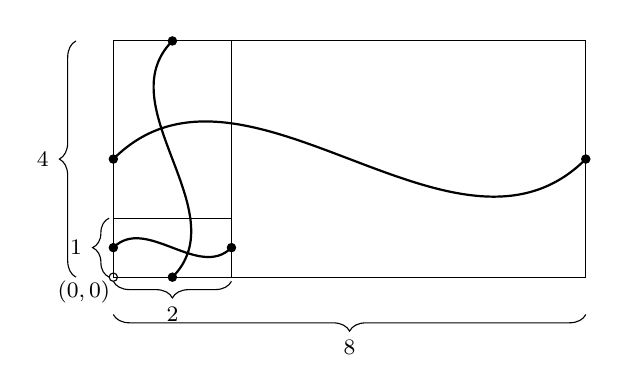
\begin{tikzpicture}[scale = 0.75]

	\draw[solid, black] (0, 0) -- (2, 0);
	\draw[solid, black] (2, 0) -- (2, 1);
	\draw[solid, black] (2, 1) -- (0, 1);
	\draw[solid, black] (0, 1) -- (0, 0);
	
	\draw[solid, black] (0, 0) -- (2, 0);
	\draw[solid, black] (2, 0) -- (2, 4);
	\draw[solid, black] (2, 4) -- (0, 4);
	\draw[solid, black] (0, 4) -- (0, 0);

	\draw[solid, black] (0, 0) -- (8, 0);
	\draw[solid, black] (8, 0) -- (8, 4);
	\draw[solid, black] (8, 4) -- (0, 4);
	\draw[solid, black] (0, 4) -- (0, 0);
	
	\draw[solid, thick, black] (0, 0.5) to[out = 45, in = -135] (2, 0.5);
	\draw[solid, thick, black] (1.0, 0) to[out = 45, in = -135] (1.0, 4);
	\draw[solid, thick, black] (0, 2.0) to[out = 45, in = -135] (8, 2.0);
	
	\draw[fill] (0, 0.5) circle (2pt);
	\draw[fill] (2, 0.5) circle (2pt);
	\draw[fill] (1,   0) circle (2pt);
	\draw[fill] (1,   4) circle (2pt);
	\draw[fill] (0,   2) circle (2pt);
	\draw[fill] (8,   2) circle (2pt);
	
	\draw[black] (0, 0) circle (2pt);
	\node[black] at (-0.5, -0.25) {{\footnotesize $(0, 0)$}};
	
	\draw [decorate, decoration = {brace, amplitude = 6pt, mirror}, xshift = 0pt, yshift = -2pt] (0, 0) -- (2, 0) node [black, midway, xshift = 0pt, yshift = -12pt] {\footnotesize $2$};
	
	\draw [decorate, decoration = {brace, amplitude = 6pt, mirror}, xshift = 0pt, yshift = -18pt] (0, 0) -- (8, 0) node [black, midway, xshift = 0pt, yshift = -12pt] {\footnotesize $8$};

	\draw [decorate, decoration = {brace, amplitude = 6pt}, xshift = -2pt, yshift = 0pt] (0, 0) -- (0, 1) node [black, midway, xshift = -12pt, yshift = 0pt] {\footnotesize $1$};

	\draw [decorate, decoration = {brace, amplitude = 6pt}, xshift = -18pt, yshift = 0pt] (0, 0) -- (0, 4) node [black, midway, xshift = -12pt, yshift = 0pt] {\footnotesize $4$};

%	
%	\draw[solid, black] (-4, -4) -- ( 4, -4);
%	\draw[solid, black] ( 4, -4) -- ( 4,  4);
%	\draw[solid, black] ( 4,  4) -- (-4,  4);
%	\draw[solid, black] (-4,  4) -- (-4, -4);
%	
%	\draw[dashed, black] (-2, -4) -- (-2, 4);
%	\draw[dashed, black] ( 2, -4) -- ( 2, 4);
%	\draw[dashed, black] (-4, -2) -- ( 4,-2);
%	\draw[dashed, black] (-4,  2) -- ( 4, 2);
%	
%	\draw[black] ( 0,  0) circle (3.35pt);
%	\node[black] at (0, -.5) {{\footnotesize $(0, 0)$}};
%	\node[black] at (-2.4, -1.65) {{\small $\Lambda_{k\phantom{2}}$}};
%	\node[black] at (-4.6, -3.65) {{\small $\Lambda_{2k}$}};
%	
%	\draw[fill] ( -1,  1) circle (3.35pt);
%	\draw[fill] ( -4,  1) circle (3.35pt);
%	
%	\draw[solid, thick, black] (-1, 1) to[out = 135, in = -45] (-4, 1);
%	
%	\draw [decorate, decoration = {brace, amplitude = 6pt, mirror}, xshift = 4pt, yshift = 0pt] (2, -2) -- (2, 2) node [black, midway, xshift = 14pt, yshift = 0pt] {\small $2k$};
%	
%	\draw [decorate, decoration = {brace, amplitude = 6pt, mirror}, xshift = 4pt, yshift = 0pt] (4, -4) -- (4, 4) node [black, midway, xshift = 14pt, yshift = 0pt] {\small $4k$};
	
\end{tikzpicture}